\documentclass[11pt,a4paper]{article}
\usepackage[margin=2.3cm]{geometry}
\IfFileExists{lmodern.sty}{\usepackage{lmodern}}{}
\usepackage[T1]{fontenc}
\usepackage{titlesec,tabularx,longtable,booktabs,array,enumitem,xcolor,fancyhdr,amsmath}
\usepackage{listings}
\usepackage{tikz}
\usetikzlibrary{arrows.meta,positioning,fit,calc,shapes.geometric,backgrounds}
\usepackage[hyphens]{url}
\usepackage{hyperref}

\definecolor{headcolor}{RGB}{15,70,60}
\definecolor{boxa}{RGB}{226,239,236}
\definecolor{boxb}{RGB}{238,242,250}
\definecolor{boxc}{RGB}{250,243,230}
\definecolor{boxd}{RGB}{245,245,245}
\definecolor{edge}{RGB}{70,70,70}
\hypersetup{colorlinks=true,linkcolor=headcolor,urlcolor=headcolor,
  pdftitle={TrustBazaar System Design - Unit 7: Disputes, Trust and Safety, Staff Tools},
  pdfauthor={S. M. Nihal Ahmed, Afrim Hossen Khan, Sabikun Nahar Sinthia}}

\titleformat{\section}{\normalfont\Large\bfseries\color{headcolor}}{\thesection}{10pt}{}
\titleformat{\subsection}{\normalfont\large\bfseries}{\thesubsection}{8pt}{}
\titleformat{\subsubsection}{\normalfont\normalsize\bfseries}{\thesubsubsection}{6pt}{}
\pagestyle{fancy}\fancyhf{}
\fancyhead[L]{System Design Document}\fancyhead[R]{Unit 7: Disputes, Trust \& Safety, Staff Tools}
\fancyfoot[C]{\thepage}\renewcommand{\headrulewidth}{0.4pt}\setlength{\headheight}{14pt}
\setlength{\emergencystretch}{3em}
\setlength{\parskip}{0.45em}\setlength{\parindent}{0pt}

\lstdefinelanguage{SQLpg}{morekeywords={CREATE,TABLE,TYPE,AS,ENUM,PRIMARY,KEY,REFERENCES,NOT,NULL,DEFAULT,CHECK,UNIQUE,INDEX,ON,WHERE,TRIGGER,BEFORE,INSERT,UPDATE,DELETE,FOR,EACH,ROW,EXECUTE,FUNCTION,RETURNS,LANGUAGE,BEGIN,END,IF,THEN,ELSE,RETURN,SELECT,FROM,INTO,ORDER,BY,DESC,LIMIT,GRANT,REVOKE,TO,SCHEMA,EXTENSION,EXISTS,OR,AND,IN,IS,ALTER,ADD,FOREIGN,GENERATED,ALWAYS,IDENTITY,DEFERRABLE,INITIALLY,DEFERRED,DECLARE,PERFORM,LOOP,RAISE,EXCEPTION,USING,DISTINCT,ROLE,LOGIN,USAGE,ALL,TABLES,STABLE,DO},sensitive=false,morecomment=[l]{--},morestring=[b]'}
\lstdefinelanguage{JS}{morekeywords={import,export,from,const,let,async,await,function,return,new,if,throw,try,catch,for,of,true,false,null},sensitive=true,morecomment=[l]{//},morestring=[b]",morestring=[b]`}
\lstset{basicstyle=\ttfamily\scriptsize,columns=fullflexible,keepspaces=true,breaklines=true,
  keywordstyle=\color{headcolor}\bfseries,commentstyle=\color{gray}\itshape,frame=single,rulecolor=\color{gray!40},
  upquote=true,literate={–}{{--}}1}

\newenvironment{dtable}[1]{\small\begin{longtable}{#1}}{\end{longtable}}

\begin{document}
\begin{titlepage}
\centering
\vspace*{1cm}
{\Large Daffodil International University}\\[0.2cm]
{\large Department of Software Engineering}\\[2cm]
\rule{\linewidth}{0.5pt}\\[0.4cm]
{\huge\bfseries System Design Document}\\[0.3cm]
{\LARGE Unit 7: Disputes, Trust \& Safety, Staff Tools}\\[0.3cm]
{\large TrustBazaar: A Verified Peer-to-Peer Auction and Marketplace Platform for Used Goods}\\[0.2cm]
\rule{\linewidth}{0.5pt}\\[1.6cm]
{\large S. M. Nihal Ahmed (232-35-002)\\[0.1cm] Afrim Hossen Khan (232-35-076)\\[0.1cm] Sabikun Nahar Sinthia (232-35-475)}\\[1.6cm]
\begin{tabular}{|l|>{\raggedright\arraybackslash}p{8cm}|}
\hline
\textbf{Status} & Draft for team review \\ \hline
\textbf{Version} & 0.1, 18 October 2026 \\ \hline
\textbf{Implements} & SRS v2.0 (\texttt{docs/srs.tex}) \\ \hline
\textbf{Depends on} & Unit 1 (Identity \& Access), Unit 2 (Order, Payment \& Escrow), Units 3 to 6 (ports and events) \\ \hline
\textbf{Database schema} & \texttt{docs/design/sql/\allowbreak 07\_disputes\_trust\_staff.sql}, tested on PostgreSQL (87 checks and concurrency tests, Appendix B) \\ \hline
\end{tabular}
\vfill
\end{titlepage}
\tableofcontents
\newpage
\section{Introduction}

\subsection{Purpose}
This document is the seventh and last backend unit of TrustBazaar's System Design Document. It covers what happens when something goes wrong, and the tools staff use to handle it:
\begin{itemize}[nosep]
  \item \textbf{disputes}: opening while the money is still held, the seller's response, the case file, the operator's decision and its execution through Unit~2's escrow;
  \item \textbf{trust \& safety}: reports, flagged activity, sanctions, seller strikes and the automatic selling suspension, and the response to a seller who recovers a sold game account;
  \item \textbf{ratings}: ratings and reviews after an order ends, and the trust summary on profiles;
  \item \textbf{staff tools}: the operator queues and the fixed list of staff actions, versioned parameters and feature switches with their validation rules, and two privacy functions (data export and lawful disclosure).
\end{itemize}
Ratings were not assigned to any unit in the original plan. They are designed here because they are a trust signal fed by the same order outcomes that disputes and strikes use.

The unit follows DC-1 to DC-14. Many earlier units already rely on it: they call \texttt{DisputeCommands}, \texttt{ReportCommands}, \texttt{SanctionPort} and \texttt{ConfigPort}, and their operator actions appear in its queues. Unit~7 is therefore mostly coordination: where a fact belongs to another unit (the dispute window, the escrow, the chat thread), Unit~7 asks that unit and does not keep a copy.

\subsection{Scope}
\textbf{In scope:} disputes and their history, statements and evidence; reports; signals for the flagged-activity queue; sanctions, strikes and restrictions; ratings, replies and removals; the staff console, the queues and the action list; parameter versions and switches; data exports and disclosures.

\textbf{Out of scope, owned by other units:} escrow movements and the fee split (Unit~2); KYC review, the NID blacklist itself, account suspension, four-eyes approvals and the audit log (Unit~1); listing review, bid voiding and auction cancellation (Unit~3); return shipments (Unit~4); game-account evidence (Unit~5); chat threads and notifications (Unit~6); the console's screens (Unit~8).

\subsection{Requirements covered}
\begin{itemize}[nosep]
  \item \textbf{Functional:} FR-DSP-01 to FR-DSP-11 (FR-DSP-12 deferred, Section~\ref{sec:review}); FR-TNS-01 to FR-TNS-09; FR-REV-01 to FR-REV-07; FR-OPS-01, FR-OPS-02, FR-OPS-08 and FR-OPS-09, completing Unit~1's FR-OPS-03 to FR-OPS-07; FR-GAM-18 (sanction and export); FR-PRV-03, FR-PRV-06.
  \item \textbf{Security:} SEC-LOG-01 (case-file views); SEC-ACC-01 to SEC-ACC-05 (staff access); SEC-IRM-04 (emergency controls); SEC-ABU-01 (reports).
  \item \textbf{Other:} NFR-USE (queue age, decision preview); DR (dispute and sanction records).
\end{itemize}

% ------------------------------------------------------------------
\section{Unit Overview}

\subsection{Responsibilities}
\begin{enumerate}[nosep]
  \item Freeze the money the moment a dispute opens, decide it on a complete case file, and execute the decision exactly once.
  \item Turn reports and signals from every unit into a small number of queues, and record every sanction with its reason and its end.
  \item Suspend selling automatically after CP-47 seller strikes, exactly once, however the strikes arrive.
  \item Show honest ratings: only from finished orders, one per direction, fixed after the edit period.
  \item Let administrators change parameters only within the SRS rules, as new versions that never alter running orders.
\end{enumerate}

\subsection{Components}
\begin{dtable}{@{}>{\raggedright\arraybackslash}p{3.8cm}>{\raggedright\arraybackslash}p{11.4cm}@{}}
\toprule
\textbf{Component} & \textbf{Responsibility} \\ \midrule \endhead
DisputeService & Opening (with the window check and the freeze), responses, evidence, withdrawal, decisions, outcome (d) (Section~\ref{sec:disputes}). \\
CaseFileBuilder & Assembles the case file from Units~2 to~6 for the assigned operator; every view audited (Section~\ref{sec:casefile}). \\
ReportService, SignalIngest & Reports from users; signals from other units' events (Section~\ref{sec:tns}). \\
SanctionService, StrikeService & Sanctions and their enforcement; strikes and the automatic suspension; implements \texttt{SanctionPort}. \\
RatingService & Eligibility from order outcomes; ratings, replies, removals; the profile summary (Section~\ref{sec:ratings}). \\
StaffConsole & Queue and action endpoints; claims with the conflict check (Section~\ref{sec:console}). \\
ConfigService & Versioned parameters and switches; validation; implements \texttt{ConfigPort} (Section~\ref{sec:config}). \\
PrivacyService & Data exports and disclosures (Section~\ref{sec:privacy}). \\
Unit7Jobs & Seller-response deadline, signal aggregation, export expiry (Section~\ref{sec:jobs}). \\
\bottomrule
\end{dtable}

\subsection{The staff console}
\label{sec:console}
FR-OPS-01 allows operators exactly eight queues, and FR-OPS-02 a closed list of actions. The console is one module that shows each queue and offers only the listed actions; the data and the action itself stay with the unit that owns them.
\begin{dtable}{@{}>{\raggedright\arraybackslash}p{4.0cm}>{\raggedright\arraybackslash}p{3.0cm}>{\raggedright\arraybackslash}p{8.2cm}@{}}
\toprule
\textbf{Queue (FR-OPS-01)} & \textbf{Owner} & \textbf{Actions offered (FR-OPS-02)} \\ \midrule \endhead
KYC submissions & Unit 1 & Approve, reject, propose revocation (four-eyes). \\
Ownership proofs & Unit 5 & Approve, reject (with the live-profile check). \\
Listings in review & Unit 3 & Approve, return, remove. \\
Reports & Unit 7 & Dismiss, or action: sanction, remove listing or review, void bid, cancel auction. \\
Flagged activity & Unit 7 (signals from Units 3--6) & Dismiss, sanction, propose blacklist; delivery issues: unlock a handover code, resolve (Unit~4). \\
Disputes & Unit 7 & Ask for information, decide, export the evidence pack. \\
Bank payout-account checks & Unit 2 & Approve, reject. \\
Payment discrepancies & Unit 2 & Resolve. \\
\bottomrule
\end{dtable}
Unit~4's delivery issues and Unit~6's chat flags appear as signals in \emph{flagged activity}, not as queues of their own, so the list stays at the eight queues the SRS allows. Two actions designed in earlier units are not in FR-OPS-02's list: unlocking a handover code and resolving a delivery issue (Unit~4). The same applies to maintaining reference data: screening and detection terms by operators, and meetup points, areas and the games catalogue by administrators. An SRS clarification adds them (I-50).

Every action requires a reason, names its object and is audited by Unit~1's \texttt{AuditService} in the same transaction (FR-OPS-07). A staff member claims a case before acting; the claim runs Unit~1's conflict check (FR-OPS-06), so an operator cannot take a dispute or report involving an account that shares their number, e-mail or NID, or one they have declared a conflict with. There is no generic create, edit or delete of users, listings, orders or payments anywhere.
\section{Interfaces}

\subsection{HTTP API}
\label{sec:api}
All paths are under \texttt{/api/v1}; policies and rate limits are those of Unit~1.

{\small
\begin{longtable}{@{}>{\ttfamily\raggedright\arraybackslash}p{1.55cm}>{\ttfamily\raggedright\arraybackslash}p{4.8cm}>{\raggedright\arraybackslash}p{2.4cm}>{\raggedright\arraybackslash}p{6.1cm}@{}}
\toprule
\textnormal{\textbf{Method}} & \textnormal{\textbf{Path}} & \textbf{Policy} & \textbf{Purpose (requirement)} \\ \midrule \endhead
\multicolumn{4}{@{}l}{\textbf{Disputes} (buyer and seller)} \\
POST & /\allowbreak orders/\allowbreak \{id\}/\allowbreak disputes & Buyer & Open: type, description (FR-DSP-01) \\
GET & /\allowbreak disputes/\allowbreak \{id\} & Buyer or seller & Status, deadlines, statements, own evidence, outcome \\
POST & /\allowbreak disputes/\allowbreak \{id\}/\allowbreak statements & Buyer or seller & Add a statement; the seller's first one is the response (FR-DSP-04) \\
POST & /\allowbreak disputes/\allowbreak \{id\}/\allowbreak evidence & Buyer or seller & Upload evidence, up to CP-33 per dispute \\
POST & /\allowbreak disputes/\allowbreak \{id\}/\allowbreak withdraw & Buyer & Withdraw before the decision (FR-DSP-10) \\
POST & /\allowbreak disputes/\allowbreak \{id\}/\allowbreak return-\allowbreak received & Seller & The returned item has arrived (outcome (d)) \\
\multicolumn{4}{@{}l}{\textbf{Reports and ratings}} \\
POST & /\allowbreak reports & SignedIn & Report a listing, user or message (FR-TNS-01) \\
POST & /\allowbreak orders/\allowbreak \{id\}/\allowbreak rating & Buyer or seller & Rate the other party (FR-REV-01) \\
PATCH & /\allowbreak ratings/\allowbreak \{id\} & Rater & Edit within the edit period (FR-REV-03) \\
POST & /\allowbreak ratings/\allowbreak \{id\}/\allowbreak reply & Rated user & One public reply (FR-REV-06) \\
GET & /\allowbreak users/\allowbreak \{id\}/\allowbreak trust & Public & Average, count, completed transactions, badges (FR-REV-04, 05) \\
\multicolumn{4}{@{}l}{\textbf{Privacy}} \\
POST & /\allowbreak me/\allowbreak data-\allowbreak export & SignedIn, StepUp & Request a copy of my data (FR-PRV-03) \\
\multicolumn{4}{@{}l}{\textbf{Staff} (operators unless stated)} \\
GET & /\allowbreak staff/\allowbreak queues/\allowbreak \{queue\} & Staff(operator) & One of the eight queues, oldest first, with age \\
POST & /\allowbreak staff/\allowbreak cases/\allowbreak \{type\}/\allowbreak \{id\}/\allowbreak claim & Staff(operator) & Claim, with the conflict check (FR-OPS-06) \\
GET & /\allowbreak staff/\allowbreak disputes/\allowbreak \{id\}/\allowbreak case-\allowbreak file & Assigned operator & The case file; each view audited (FR-DSP-05) \\
POST & /\allowbreak staff/\allowbreak disputes/\allowbreak \{id\}/\allowbreak request-\allowbreak info & Assigned operator & Ask the seller for more (FR-DSP-09) \\
POST & /\allowbreak staff/\allowbreak disputes/\allowbreak \{id\}/\allowbreak decision & Assigned operator & Decide; proposes four-eyes approval when CP-30 applies (FR-DSP-06) \\
POST & /\allowbreak staff/\allowbreak reports/\allowbreak \{id\}/\allowbreak resolution & Assigned operator & Dismiss or action, with a reason \\
POST & /\allowbreak staff/\allowbreak signals/\allowbreak \{id\}/\allowbreak review & Staff(operator) & Dismiss or action \\
POST, DELETE & /\allowbreak staff/\allowbreak users/\allowbreak \{id\}/\allowbreak sanctions & Staff(operator) & Apply or lift a sanction (FR-TNS-03) \\
POST & /\allowbreak staff/\allowbreak ratings/\allowbreak \{id\}/\allowbreak removal & Staff(operator) & Remove a review breaking the policy (FR-REV-07) \\
GET & /\allowbreak staff/\allowbreak disputes/\allowbreak \{id\}/\allowbreak evidence-\allowbreak pack & Assigned operator & Export for law enforcement (FR-GAM-18) \\
POST & /\allowbreak staff/\allowbreak disclosures & Staff(operator) & Record a lawful request; proposes four-eyes (FR-PRV-06) \\
GET, POST & /\allowbreak admin/\allowbreak config & Staff(admin) & Current version; publish a change (FR-OPS-03, 08, 09) \\
\bottomrule
\end{longtable}
}

\subsection{Ports provided}
\begin{lstlisting}[language=Java,morekeywords={interface,type,Promise,string,boolean,number,bigint}]
interface DisputeCommands {                       // used by Unit 5, in its own transaction (DC-13)
  open(o: { orderId: string; type: DisputeType; description: string; by: 'buyer' | 'system' },
       tx: EntityManager): Promise<string>;        // credentials_invalid report, re-key overdue
}
interface ReportCommands {                        // used by Unit 6 (FR-CHT-06)
  report(r: { reporterId: string; target: ReportTarget; category: ReportCategory; text?: string }): Promise<string>;
}
interface SanctionPort {                          // used by Unit 1 (assertCanTransact) and Unit 2 (payouts)
  restrictions(userId: string): Promise<{ canSell: boolean; canBuyBid: boolean; fraudHold: boolean }>;
}
interface ConfigPort {                            // used by every unit (DC-9)
  current(): Promise<{ version: number; get<T>(code: string): T }>;
  atVersion(version: number): Promise<{ get<T>(code: string): T }>;   // a running order's own values
}
interface TrustQuery {                            // used by Units 3 and 8
  profileSummary(userId: string): Promise<{ averageRating: number | null; ratingCount: number;
                                            completedTransactions: number }>;
}
\end{lstlisting}

\subsection{Events}
\begin{dtable}{@{}>{\raggedright\arraybackslash}p{6.2cm}>{\raggedright\arraybackslash}p{9.0cm}@{}}
\toprule
\textbf{Event} & \textbf{Use} \\ \midrule \endhead
\multicolumn{2}{@{}l}{\textit{Published (outbox, DC-6)}} \\
\texttt{disputes.dispute.opened}, \texttt{.withdrawn}, \texttt{.decided} & Notifications to both parties (FR-DSP-03, FR-DSP-07); Unit~6 holds or releases the chat thread. \\
\texttt{trust.sanction.applied}, \texttt{.lifted} & Notifications with the reason (FR-TNS-03); Unit~3 hides or shows listings. \\
\texttt{trust.report.resolved} & Notification to the reporter: reviewed, and whether action was taken (FR-TNS-09). \\
\texttt{staff.config.published} & Every unit refreshes its cached parameters. \\
\multicolumn{2}{@{}l}{\textit{Consumed (idempotent)}} \\
\texttt{orders.escrow.released}, \texttt{.refunded}, \texttt{.partially\_refunded} & Rating eligibility (FR-REV-01); a refund at a missed fulfilment deadline is a seller strike (FR-TNS-04). \\
\texttt{orders.order.cancelled\_by\_seller} & Seller strike (FR-PAY-09, FR-TNS-04). \\
\texttt{delivery.return.delivered} & Outcome (d) completed. \\
\texttt{auctions.flag.raised}, \texttt{listings.\allowbreak listing.\allowbreak relisting\_flagged} (new, I-45), \texttt{chat.message.flagged}, \texttt{delivery.issue.opened} (new, I-46) & Signals in the flagged-activity queue (Section~\ref{sec:signals}). \\
\texttt{identity.account.closed} & Pending exports cancelled; ratings by the user shown as ``Closed account''. \\
\bottomrule
\end{dtable}

\subsection{Ports required}
\begin{dtable}{@{}>{\raggedright\arraybackslash}p{4.6cm}>{\raggedright\arraybackslash}p{10.6cm}@{}}
\toprule
\textbf{Port} & \textbf{Provider and use} \\ \midrule \endhead
\texttt{IdentityCommands}, \texttt{ApprovalService}, \texttt{AuditService}, \texttt{StaffQuery}, \texttt{FileVault} (Unit 1) & Account suspension and reinstatement; four-eyes; audit; conflict check; encrypted evidence files. \\
\texttt{OrdersPort}, \texttt{EscrowQuery}, \texttt{EscrowCommands} (Unit 2) & Order facts and lock (DC-14); \texttt{disputeAllowed}; \texttt{freezeForDispute}, \texttt{applyDisputeOutcome}, \texttt{withdrawDispute}; outcome preview from \texttt{payments.split}. \\
\texttt{ListingsCommands} (Unit 3) & Remove a listing for a sanction. \\
\texttt{DeliveryQueries}, \texttt{DeliveryCommands} (Unit 4) & \texttt{notReceivedAllowed}; the fulfilment record; \texttt{quoteReturn}, \texttt{bookReturn}. \\
\texttt{GameAccountQueries} (Unit 5) & \texttt{credentialsInvalidAllowed}; \texttt{evidence}. \\
\texttt{ChatCommands}, \texttt{Notifier} (Unit 6) & Holds and the staff read; notices to parties and reporters. \\
\bottomrule
\end{dtable}
\section{Data Design}
\label{sec:data}
The schema is in \texttt{docs/design/sql/07\_disputes\_trust\_staff.sql} (Appendix~\ref{app:ddl}), loaded after Units~1 to~6. The unit owns three schemas: \texttt{disputes}, \texttt{trust} and \texttt{staff}. Their foreign keys point only to users, staff accounts and approvals (Unit~1) and to orders (Unit~2), as DC-5 allows. Listings, threads and messages are referred to by identifier only. No function reads another unit's tables (DC-1). Facts that belong to other units, such as ``the dispute window is open'' or ``the order's escrow is \texttt{held}'', arrive as arguments that the service obtained from the owning unit's port in the same transaction.

\tikzset{
  ent/.style={draw=edge, fill=white, rounded corners=1.5pt, align=left, inner sep=3pt, font=\sffamily\scriptsize, text width=3.9cm},
  fk/.style={-{Latex[length=1.6mm]}, draw=edge!80, semithick},
}
\newcommand{\ent}[2]{\textbf{\color{headcolor}#1}\\[-1pt]{\ttfamily\tiny #2}}
\begin{figure}[!htbp]
\centering
\resizebox{0.98\textwidth}{!}{%
\begin{tikzpicture}
\node[ent, fill=boxd] (ord) at (5.2,6.4) {\ent{orders.orders}{(Unit 2)}};
\node[ent, fill=boxa, text width=4.4cm] (d) at (5.2,3.6) {\ent{disputes.disputes}{order, buyer, seller, item\_kind, type\\description, item\_price, amount\_collected\\status, opened\_by, seller\_due\_at\\info\_due\_at, decision\_target\_at\\assigned\_to, outcome, item\_refund\\return\_fare, payer, reason, approval\\last actor and reason\\one open per order}};
\node[ent] (h) at (0,5.2) {\ent{history}{from, to, actor, reason, at\\(append-only, by trigger)}};
\node[ent] (st) at (0,3.4) {\ent{statements}{party, text, at (append-only)}};
\node[ent] (ev) at (0,1.6) {\ent{evidence}{party, storage\_key, sha256\\mime, size (CP-33)\\at most 10 (append-only)}};
\node[ent, fill=boxb] (rep) at (10.4,6.4) {\ent{trust.reports}{reporter, target, message\\subject\_user, category\\status, resolution\\one open per reporter and target}};
\node[ent, fill=boxb] (sig) at (10.4,4.3) {\ent{trust.signals}{kind, source\_ref (unique)\\subject\_user, detail, status}};
\node[ent, fill=boxb] (san) at (10.4,2.0) {\ent{trust.sanctions}{user, kind, reason, fraud\\starts, ends (or until review)\\automatic, listing, related\\lifted, lift approval\\(never deleted)}};
\node[ent, fill=boxb] (str) at (5.2,0.4) {\ent{trust.strikes}{user, reason, order\\once per order and reason\\(append-only)}};
\node[ent, fill=boxb] (el) at (15.6,5.6) {\ent{trust.rating\_eligibility}{order PK, buyer, seller\\closed\_at, rate\_until\\completed}};
\node[ent, fill=boxb] (rt) at (15.6,3.0) {\ent{trust.ratings}{order, rater, ratee, stars, text\\edit\_until, reply, removal\\one per direction}};
\node[ent, fill=boxc] (cv) at (20.8,6.4) {\ent{staff.config\_versions}{version PK, by, reason\\approval (append-only)}};
\node[ent, fill=boxc] (cval) at (20.8,4.3) {\ent{staff.config\_values}{(version, code) PK\\value jsonb (append-only)}};
\node[ent, fill=boxc] (dis) at (20.8,2.2) {\ent{staff.disclosures}{subject, authority\\legal\_reference, scope\\approval, notified / withheld}};
\node[ent, fill=boxc] (exr) at (20.8,0.4) {\ent{staff.export\_requests}{user, requested, ready\\file\_key, expires\\one pending per user}};
\draw[fk] (d.north) -- (ord.south);
\draw[fk] (h.east) -- ++(0.35,0) |- ([yshift=22pt]d.west);
\draw[fk] (st.east) -- ([yshift=-6pt]d.west|-st.east);
\draw[fk] (ev.east) -- ++(0.35,0) |- ([yshift=-30pt]d.west);
\draw[fk, dashed] (d.south) -- (str.north);
\draw[fk] (str.east) -- ++(1.0,0) |- (ord.east);
\draw[fk] (rt.north) -- (el.south);
\draw[fk] (cval.north) -- (cv.south);
\end{tikzpicture}}
\caption{The schemas of Unit~7. Users and staff accounts (Unit~1) are referenced by most tables; disputes, sanctions, parameter versions and disclosures also reference Unit~1's approvals, and rating eligibility references the order. Those arrows are omitted. A strike references its order only; the dashed arrow shows that a lost dispute creates one.}
\label{fig:er}
\end{figure}

\subsection{Tables and rules the database enforces}
\begin{dtable}{@{}>{\ttfamily\raggedright\arraybackslash}p{3.6cm}>{\raggedright\arraybackslash}p{11.6cm}@{}}
\toprule
\textnormal{\textbf{Table}} & \textbf{Rules enforced by the database} \\ \midrule \endhead
disputes & Buyer and seller differ. The type fits the item: game-account types only for game accounts, physical types only for physical items (FR-DSP-01). A description of at least 20 characters. One open dispute per order (FR-DSP-11). A dispute starts as \texttt{open}, and a type that was withdrawn on the order cannot be opened again (FR-DSP-10). What the dispute is about (order, parties, type, description, amounts, opening) is fixed. Only the transitions of Figure~\ref{fig:states}. Every status change names its actor and reason. A decision needs an outcome, the operator, the time and a reason of at least 20 characters, and is final. A partial refund is above zero and below the item price (FR-PAY-11); a refund after return names the fare and who pays it. A decision on BDT~20{,}000 or more needs an executed four-eyes approval (CP-30). \\
history & One row for every status change, written by a trigger, so it cannot be skipped (FR-DSP-09). Append-only. \\
statements, evidence & Append-only. Evidence: the allowed file types, at most 10~MB each, at most 10 per dispute (CP-33), and only while the dispute is being considered. \\
reports & A user cannot report themselves. A reported message names the message. One open report per reporter and target. A resolution records the operator, the time and a reason. \\
signals & One row per source event (kind and source reference unique), so an event delivered twice is stored once. A review records the operator. \\
sanctions & A reason of at least 10 characters. A warning and a listing removal have no duration; a listing removal names the listing. A sanction applied by an operator names the operator. A sanction cannot be rewritten: its end changes only by lifting it, with a reason; lifting an account suspension needs four-eyes approval (CP-30). At most one live automatic suspension per user. Never deleted. \\
strikes & One strike per order and reason. Append-only. \\
rating\_eligibility, ratings & A rating exists only for an order in \texttt{rating\_eligibility}, that is, one whose escrow reached a terminal state (FR-REV-02). Only the buyer and the seller rate each other, once in each direction, within the CP-39 window. 1--5 stars. Stars and text change only within the edit period and are then fixed (FR-REV-03). One reply, only to a written review, never changed (FR-REV-06). A removal records the operator and a reason, and is final (FR-REV-07). \\
config\_versions, config\_values & Append-only. A code is a CP or SW identifier. Version~1 is the seed; every later version names its administrator and a reason. \\
disclosures & Nothing is disclosed without an approval. The user is either told, or the reason not to tell is recorded (FR-PRV-06). \\
export\_requests & One export in preparation per user. A ready export has its file and its expiry. \\
\bottomrule
\end{dtable}
The application role cannot update or delete the history, statements, evidence, strikes or parameter versions, and cannot delete sanctions (tested).

% ------------------------------------------------------------------
\section{Disputes}
\label{sec:disputes}

\subsection{Life cycle}
\begin{figure}[!htbp]
\centering
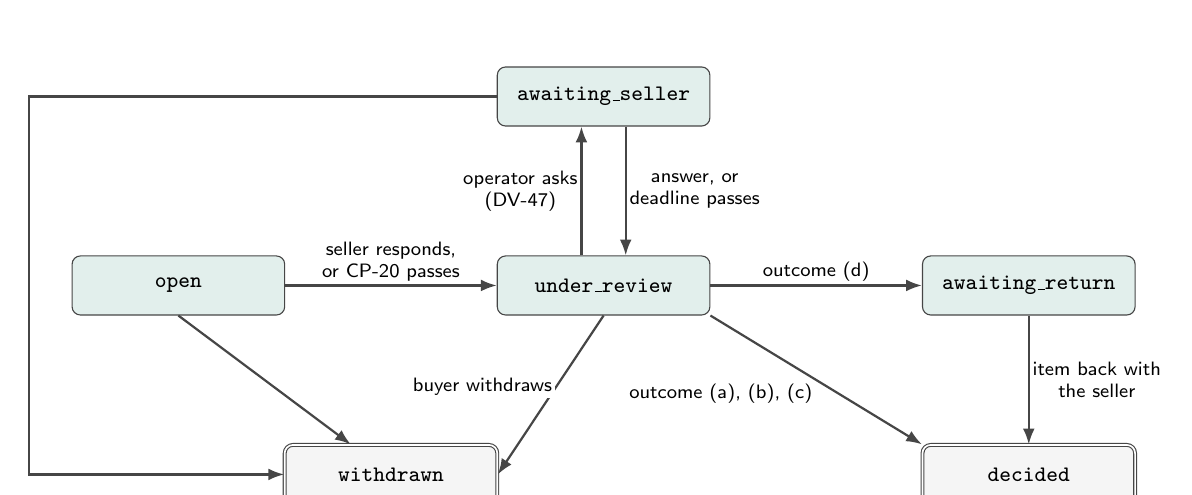
\begin{tikzpicture}[
  font=\sffamily\footnotesize,
  st/.style={draw=edge, rounded corners=3pt, fill=boxa, minimum width=2.7cm, minimum height=0.75cm, align=center},
  fin/.style={st, fill=boxd, double},
  tr/.style={-{Latex[length=2mm]}, draw=edge, thick},
  lab/.style={font=\sffamily\scriptsize, align=center, fill=white, inner sep=1pt}
]
\node[st] (open) at (0,0) {\texttt{open}};
\node[st] (rev) at (5.4,0) {\texttt{under\_review}};
\node[st] (aws) at (5.4,2.4) {\texttt{awaiting\_seller}};
\node[st] (awr) at (10.8,0) {\texttt{awaiting\_return}};
\node[fin] (dec) at (10.8,-2.4) {\texttt{decided}};
\node[fin] (wd) at (2.7,-2.4) {\texttt{withdrawn}};
\draw[tr] (open) -- node[lab, above]{seller responds,\\or CP-20 passes} (rev);
\draw[tr] ([xshift=-8pt]rev.north) -- node[lab, left]{operator asks\\(DV-47)} ([xshift=-8pt]aws.south);
\draw[tr] ([xshift=8pt]aws.south) -- node[lab, right]{answer, or\\deadline passes} ([xshift=8pt]rev.north);
\draw[tr] (rev) -- node[lab, above]{outcome (d)} (awr);
\draw[tr] (rev.south east) -- node[lab, pos=0.5, below left]{outcome (a), (b), (c)} (dec.north west);
\draw[tr] (awr) -- node[lab, right]{item back with\\the seller} (dec);
\draw[tr] (open.south) -- (wd);
\draw[tr] (rev.south) -- node[lab, pos=0.45, left]{buyer withdraws} (wd.east);
\draw[tr] (aws.west) -| (-1.9,-2.4) -- (wd.west);
\end{tikzpicture}
\caption{Dispute statuses (FR-DSP-09). The buyer can withdraw from \texttt{open}, \texttt{under\_review} and \texttt{awaiting\_seller}. Every arrow writes a history row with its actor and reason.}
\label{fig:states}
\end{figure}

The six statuses are the SRS's (FR-DSP-09). While the dispute is \texttt{open}, the seller has CP-20 (48~hours) to respond. The review starts when the seller responds, or when CP-20 passes without a response, in which case the operator decides on the evidence available (FR-DSP-04). The review start sets the decision target, CP-21 after it (FR-DSP-08). The queue shows the age of each dispute and puts overdue ones first (DV-52). During the review the operator may ask the seller for more; the dispute is then \texttt{awaiting\_seller} until the seller answers or the operator's deadline passes (DV-47, 24~hours), and returns to review either way. The decision target is not reset by such a request: the CP-21 clock measures the operator, not the seller.

\subsection{Opening}
\label{sec:opening}
The buyer opens a dispute from the order view with a type, a description and evidence (FR-DSP-01). Two kinds of dispute are opened by the system rather than the buyer: Unit~5 opens a \texttt{credentials\_invalid} dispute when the buyer reports that the credentials do not work (FR-GAM-14), and when the seller does not answer a re-key in time (DV-37). Both go through \texttt{DisputeCommands.open}. Who may open which type, and when, is decided by the unit that owns the deadline:
\begin{dtable}{@{}>{\ttfamily\raggedright\arraybackslash}p{3.3cm}>{\raggedright\arraybackslash}p{5.4cm}>{\raggedright\arraybackslash}p{6.5cm}@{}}
\toprule
\textnormal{\textbf{Type}} & \textbf{Window (SRS)} & \textbf{Answered by} \\ \midrule \endhead
not\_as\_described, damaged, other (physical) & CP-18 after the delivery event & Unit~2 \texttt{EscrowQuery.disputeAllowed}: \texttt{held} and inside the window. \\
not\_received & CP-17 after pickup with no delivery (FR-DLV-11) & Unit~4 \texttt{notReceivedAllowed}, and Unit~2 for \texttt{held}. \\
credentials\_invalid & The takeover window, until the buyer confirms the new recovery e-mail (FR-GAM-14) & Unit~5 \texttt{credentials\-Invalid\-Allowed}, and Unit~2 for \texttt{held}. Opened by Unit~5 itself. \\
seller\_recovery, other (game) & The protection period CP-24 (FR-GAM-16) & Unit~2 \texttt{disputeAllowed}. \\
\bottomrule
\end{dtable}
After the payment has been released or refunded, no dispute can be opened; later complaints are reports (FR-DSP-11). A seller who recovers an account after release is handled through a report and the sanction of Section~\ref{sec:gam18}.

Opening is one transaction, with the locks in the order of DC-14, the dispute row taking the place of the delivery row:
\begin{enumerate}[nosep]
  \item lock the order through \texttt{OrdersPort.lockForFulfilment}, which also gives the parties, the item kind and the amounts;
  \item ask the owning unit whether this type may be opened now (table above);
  \item \texttt{disputes.open}, which inserts the dispute (refused if one is open, or if this type was withdrawn), writes the first history row and the \texttt{disputes.dispute.opened} event;
  \item \texttt{EscrowCommands.freezeForDispute}: the escrow moves to \texttt{frozen\_disputed}, which stops every automatic release (FR-DSP-02);
  \item \texttt{ChatCommands.hold} on the order's thread, so it is kept and the assigned operator may read it (FR-CHT-10);
  \item the evidence files, already uploaded to Unit~1's \texttt{FileVault} with the evidence purpose, are recorded.
\end{enumerate}
If any step fails, nothing is kept: no dispute without a frozen escrow, and no frozen escrow without a dispute. Ten simultaneous openings on one order produced one dispute and nine refusals (Section~\ref{sec:testing}). The event notifies the seller (FR-DSP-03) and the dispute appears in the queue.

\subsection{The seller's response and the parties' statements}
The seller's first statement is the response: it moves the dispute to review (FR-DSP-04). Either party may add statements and evidence until the decision, up to CP-33 (10) files per dispute in total. A response after CP-20 is refused, and the review starts on the evidence available. The CP-20 job checks every five minutes; a seller who answers one minute after the deadline is refused even if the job has not yet run, because the function compares the time itself.

\subsection{The case file}
\label{sec:casefile}
The assigned operator sees one case file (FR-DSP-05). Each item comes from the unit that owns it, through its port; Unit~7 keeps no copies.
\begin{dtable}{@{}>{\raggedright\arraybackslash}p{5.0cm}>{\raggedright\arraybackslash}p{3.0cm}>{\raggedright\arraybackslash}p{7.2cm}@{}}
\toprule
\textbf{Item (FR-DSP-05)} & \textbf{Unit} & \textbf{Source} \\ \midrule \endhead
The order and the listing as they were at the time of sale & 2 & The order with its listing snapshot (Unit~2 stores the snapshot at checkout). \\
The escrow history & 2 & \texttt{EscrowQuery.getEscrow}, with its state changes. \\
The settlement and ledger entries & 2 & The order's ledger entries and the preview of each outcome from \texttt{payments.split}, so the operator sees the exact amounts before deciding. \\
The delivery or handover records & 4 & \texttt{fulfilmentRecord}: proposals, code entries (never the code), shipments, courier history, issues. \\
The chat thread for the listing & 6 & \texttt{chat.staff\_read}, allowed only by the dispute's own hold; each read logged. \\
Both parties' evidence & 7 & Statements and evidence; files through \texttt{FileVault} signed links (CP-31). \\
For game accounts: the ownership proof, takeover confirmations and credential-access log & 5 & \texttt{GameAccountQueries.evidence}. Never the credentials. \\
Context (not in the SRS list) & 7 & Earlier disputes, strikes and sanctions of both parties. \\
\bottomrule
\end{dtable}
Personal data in the case file is masked by default (SEC-ACC-05). Every view of the case file is written to the audit log (SEC-LOG-01). Only the operator assigned to the dispute can open it, and assignment passes Unit~1's conflict check (FR-OPS-06). In the race test, ten operators claimed one dispute at once; one got it and nine were refused.

\subsection{Decision and execution}
\label{sec:decision}
The operator chooses one of the four outcomes of FR-DSP-06 and writes a reason; the parties see the reason (FR-DSP-07). The service executes the decision in one transaction, locking the order, then the dispute, then the escrow:
\begin{dtable}{@{}>{\raggedright\arraybackslash}p{3.4cm}>{\raggedright\arraybackslash}p{11.8cm}@{}}
\toprule
\textbf{Outcome} & \textbf{Execution} \\ \midrule \endhead
(a) Release & \texttt{disputes.decide}, then \texttt{applyDisputeOutcome(release)}: the seller is paid as on a normal release. \\
(b) Full refund & \texttt{applyDisputeOutcome(full)}. Unit~2 refunds the item price, and the delivery fee too if the courier never picked up. \\
(c) Partial refund & \texttt{applyDisputeOutcome(partial, itemRefund)}, with the item refund above zero and below the item price (FR-PAY-11). \\
(d) Refund after return & \texttt{DeliveryCommands.quoteReturn} and \texttt{bookReturn} with the payer the operator chose; \texttt{applyDisputeOutcome(after\_return)} keeps the escrow frozen. The dispute is \texttt{awaiting\_return}. When Unit~4 reports \texttt{delivery.return.delivered}, or the seller records receipt, \texttt{return\_completed} closes it and Unit~2 makes the refund (I-44). \\
\bottomrule
\end{dtable}
Any outcome other than release is a lost dispute for the seller, and records a strike (FR-TNS-04, Section~\ref{sec:strikes}) in the same transaction. A partial refund counts as lost, because the buyer's complaint was found at least partly justified. The \texttt{disputes.dispute.decided} event notifies both parties and releases the chat hold.

A decision cannot be changed. Neither the operator nor anyone else can change the outcome, the amounts or the reason afterwards; the database refuses it.

\subsection{Four-eyes approval}
\label{sec:foureyes}
CP-30 requires four-eyes approval for ``dispute outcomes of BDT 20{,}000 or more''. The design applies the threshold to the amount the buyer paid (\texttt{amount\_collected}), because that is what any outcome can move. For such a dispute, the decision endpoint does not decide: it proposes the decision through Unit~1's \texttt{ApprovalService} (action \texttt{dispute.outcome\_20000}, with the outcome, amounts and reason as the payload). A second operator who is not the proposer approves it, and the approval's handler, registered by Unit~7, runs the decision with the approval's identifier in the approval's transaction. Without an executed approval the database refuses the decision (tested). Until the approval, the dispute stays \texttt{under\_review} and the buyer can still withdraw; if the buyer withdraws, the approval fails when it runs, because the dispute is no longer under review.

\subsection{Withdrawal}
The buyer may withdraw before the decision (FR-DSP-10). In one transaction: \texttt{disputes.withdraw}; \texttt{EscrowCommands.\allowbreak withdrawDispute}, which returns the escrow to \texttt{held} with automatic release at the later of the original time and 24~hours after the withdrawal; for game accounts, \texttt{GameAccountCommands.disputeWithdrawn}, which returns the handover to its state before the dispute; and the release of the chat hold. A withdrawn type cannot be opened again on that order, but another type can (tested).

Decision and withdrawal can arrive at the same moment. Both lock the dispute row, and whichever comes second finds the dispute closed and is refused. In the race test, 20 disputes were each decided and withdrawn at once: every dispute ended either decided or withdrawn, never both, never neither.

\subsection{Review of a decision (FR-DSP-12, deferred)}
\label{sec:review}
FR-DSP-12 (a Could requirement) lets a party ask for one review of a decision by a different operator within three days. It is deferred. A decision is executed at once, so the escrow is already released or refunded when a review could be asked for, and a changed outcome would have to take money back from a party who may already have withdrawn it. Doing this properly needs either a delay before every execution, which slows every dispute, or a recovery process through Unit~2's \texttt{seller\_receivable}, which only works in one direction. The schema keeps the decision final; adding the review later means a new \texttt{review\_requested} status before execution, and does not change any other table. This is listed as an SRS clarification (I-50).
\section{Trust \& Safety}
\label{sec:tns}

\subsection{Reports}
Any registered user can report a listing, a user or a chat message as fraudulent, counterfeit, prohibited, misrepresented or abusive (FR-TNS-01); chat reports arrive through \texttt{ReportCommands} (FR-CHT-06). The report names the user it is about, so the queue can group reports by user, and the conflict check can be made at claim. A reporter may have one open report per target; a second one adds nothing and is refused, which stops one person from pushing a listing up the queue. Reports are also rate-limited by CP-35 (20 a day). A report on a message or thread places a hold on the thread (Unit~6), so the assigned operator may read it.

The operator resolves a report as \emph{dismissed} or \emph{actioned}, with a reason. Actions are those of FR-OPS-02: a sanction, removing the listing or a review, voiding a bid, or cancelling an auction; each is carried out by the owning unit. The \texttt{trust.report.resolved} event tells the reporter that the report was reviewed and whether action was taken, without the details of any sanction (FR-TNS-09). The text is the same for every kind of action: ``Thank you. We reviewed your report and took action'' or ``\dots{} and found no breach of our rules''.

\subsection{Flagged activity}
\label{sec:signals}
The flagged-activity queue holds \emph{signals}: things another unit noticed that an operator should look at. A signal is stored once per source event, however often the event is delivered.
\begin{dtable}{@{}>{\raggedright\arraybackslash}p{4.0cm}>{\raggedright\arraybackslash}p{2.0cm}>{\raggedright\arraybackslash}p{9.2cm}@{}}
\toprule
\textbf{Signal} & \textbf{From} & \textbf{Meaning} \\ \midrule \endhead
Shill bidding & Unit 3 & The shill score of an auction (FR-AUC-18), including bidders linked to the seller (FR-TNS-08). \\
Relisting & Unit 3 & A similar item relisted shortly after a cancelled or disputed sale (FR-TNS-02). \\
Linked accounts & Units 1, 2 & Accounts sharing a device, a payout account or a payment instrument (FR-TNS-08), from a daily check through their query ports. \\
Chat & Unit 6 & Off-platform or credential warnings, aggregated per user per day (DV-51): one signal, with the count, rather than one per message. \\
Delivery issue & Unit 4 & A handover locked by wrong codes, or a courier problem. The operator unlocks or resolves it through Unit~4's actions. \\
\bottomrule
\end{dtable}
An operator dismisses a signal or acts on it, with a note. Acting usually means a sanction, or proposing a blacklist entry through Unit~1.

\subsection{Sanctions}
\label{sec:sanctions}
An operator may apply the five sanctions of FR-TNS-03. Each has a reason, and an end date or ``until review'' (no end), and the user is told the reason. The restrictions are computed from the live sanctions by \texttt{trust.restrictions}, which \texttt{SanctionPort} exposes. Each unit applies them where it acts:
\begin{dtable}{@{}>{\raggedright\arraybackslash}p{3.3cm}>{\raggedright\arraybackslash}p{11.9cm}@{}}
\toprule
\textbf{Sanction} & \textbf{Effect and where it is enforced} \\ \midrule \endhead
Warning & A notice only. Recorded, so it appears in the case files of later disputes. \\
Listing removal & Unit~3 removes the listing (\texttt{ListingsCommands}); a notice with the reason. \\
Selling suspended & No new listings, and the user's listings hidden (Unit~3, on \texttt{trust.sanction.applied}). Unit~1's \texttt{assertCanTransact} refuses selling actions using \texttt{SanctionPort}. \\
Buying suspended & No bids or purchases: Unit~1's \texttt{assertCanTransact}, called by Units~2 and~3. \\
Account suspended & All of the above, and Unit~1's \texttt{suspendAccount}, which ends the user's sessions. Lifting it needs four-eyes approval (CP-30), through \texttt{reinstateAccount}. \\
Fraud flag (any suspension) & Payouts to the user are held until an operator reviews them (FR-TNS-05): Unit~2's payout job asks \texttt{SanctionPort} for \texttt{fraudHold}. \\
\bottomrule
\end{dtable}
Orders already paid continue to completion under the normal escrow rules (FR-TNS-05): a suspended seller still has to deliver, and a suspended buyer can still confirm receipt or open a dispute. A sanction cannot be edited. Shortening or ending it is a lift, with a reason; a different sanction is a new one. Expired sanctions stop counting by themselves, without a job (tested).

\subsection{Seller strikes and the automatic suspension}
\label{sec:strikes}
A seller gets a strike for each of the three events of FR-TNS-04:
\begin{itemize}[nosep]
  \item a unilateral cancellation after payment (\texttt{orders.order.cancelled\_by\_seller}, FR-PAY-09);
  \item a missed fulfilment deadline (the refund event of Unit~2 with that reason, I-44);
  \item a lost dispute (Section~\ref{sec:decision}).
\end{itemize}
A strike is stored once per order and reason, so a repeated event adds nothing. \texttt{trust.\allowbreak record\_strike} counts the seller's strikes in the CP-47 window (90 days). At the CP-47 count (3), it applies a \texttt{selling\_suspended} sanction marked automatic, ``until review''. It does so once: further strikes while that suspension is live add strikes but no second suspension. The function holds a lock for the seller while it counts. In the race test, ten strikes for one seller arrived at once; the result was ten strikes and exactly one suspension. An operator reviews the automatic suspension from the flagged-activity queue and lifts it or replaces it with a decided sanction.

Unit~3's bidder strikes for unpaid auction wins (CP-12) are a different thing: they restrict bidding, are kept by Unit~3, and do not count here.

\subsection{A seller who recovers a sold game account}
\label{sec:gam18}
When an operator confirms that a seller recovered a sold account (FR-GAM-18), either by deciding a \texttt{seller\_recovery} dispute for the buyer or by actioning a report after release, the console runs three steps:
\begin{enumerate}[nosep]
  \item an \texttt{account\_suspended} sanction with the fraud flag, at once, which also holds the seller's payouts;
  \item \texttt{IdentityCommands.proposeBlacklist} with the order and the reason, so that the seller's NID blind index is added to the blacklist when a second staff member approves (FR-TNS-06, CP-30);
  \item the evidence pack: the ownership proof, the credential-access log and the takeover confirmations (Unit~5's \texttt{evidence}), and the dispute's history, statements and evidence. It is one PDF with a hash list of the files, created on request and audited, and served by a signed link.
\end{enumerate}

% ------------------------------------------------------------------
\section{Ratings}
\label{sec:ratings}
When an order's escrow reaches a terminal state (released, refunded or partially refunded), the Unit~2 event creates its row in \texttt{rating\_eligibility}, with the CP-39 window (14 days). Only then can the buyer and the seller rate each other, once each, with 1--5 stars and optional text (FR-REV-01, FR-REV-02). An order that was never paid never reaches a terminal escrow state and so can never be rated. A rating can be edited for 48~hours (CP-39) and is then fixed (FR-REV-03). The rated user may post one reply to a written review (FR-REV-06, Could). An operator may remove a review that breaks the content policy, with a reason; it then no longer counts (FR-REV-07).

The profile summary shows the average of the ratings not removed, their number, and the number of completed transactions (FR-REV-04): orders released to the seller, where the user was either party. Refunded orders can be rated, but do not count as completed. The verified and Pro badges (FR-REV-05) come from Unit~1 and Unit~2 and are added by the API. Ratings are shown with the rater's name, or ``Closed account''.

% ------------------------------------------------------------------
\section{Parameters and Feature Switches}
\label{sec:config}
Every configurable parameter of the SRS (CP-01 to CP-47) and the two emergency switches of SEC-IRM-04 (\texttt{SW-new\_orders}, \texttt{SW-payouts}) live in one versioned set. Version~1 is seeded with the SRS defaults. An administrator changes the set by publishing a new version: the previous values with the changes applied (FR-OPS-03). Versions are never edited (FR-OPS-08).
\begin{itemize}[nosep]
  \item \textbf{Validation} (FR-OPS-09). \texttt{staff.config\_violations} checks the complete candidate set against every rule of the SRS parameter table, including rules between parameters (CP-19 longer than CP-18; Pro commission not above standard; Pro limit not below standard; the CP-30 list may only grow). All broken rules are reported together. An unknown parameter is refused.
  \item \textbf{Four-eyes.} A change to a switch, to CP-36 (the game-account feature) or to CP-30 needs an executed approval (SEC-IRM-04, CP-30). The proposal goes through \texttt{ApprovalService}; the handler publishes the version with the approval.
  \item \textbf{Running items keep their values.} Units~2 and~3 store the version on each order, listing and auction at creation, and read their values through \texttt{ConfigPort.atVersion} (FR-OPS-08). New items use \texttt{current}.
  \item \textbf{Caching.} Each instance caches the current version, and refreshes on \texttt{staff.\allowbreak config.\allowbreak published} and at least every 60~seconds (DV-50). A new order may therefore be created on the previous version for up to a minute after a change. This is acceptable, because the order keeps whichever version it was created with. The emergency switches are the exception: they are read without the cache, so that stopping new orders takes effect at once.
\end{itemize}
Publishing takes a lock, so concurrent publications produce consecutive versions, each complete (tested with ten at once). The other administrator actions of FR-OPS-03 (staff accounts, MFA resets, the audit-log view) are Unit~1's.

% ------------------------------------------------------------------
\section{Privacy Functions}
\label{sec:privacy}
\textbf{Data export} (FR-PRV-03, Should). A signed-in user, after step-up, requests a copy of their data. A job collects it through each unit's export query: profile and consents (Unit~1), orders and payments (Unit~2), listings and bids (Unit~3), addresses and shipments (Unit~4), game-account listings and handovers without any credential (Unit~5), own chat messages and notifications (Unit~6), and own disputes, reports, ratings and sanctions (Unit~7). The result is one JSON file in a ZIP, stored encrypted, offered through a signed link for 7 days (DV-49). One export may be in preparation at a time, and one may be requested every 7 days. KYC images are not included; the export says they can be requested from the operator.

\textbf{Lawful disclosure} (FR-PRV-06). An operator records a request from an authority with its legal reference and its scope. Nothing is disclosed until a second staff member approves it (four-eyes, recorded in Unit~1). The user is told, unless the law forbids it; then the reason is recorded instead. Both steps are audited.
\section{Scheduled Jobs and Event Consumers}
\label{sec:jobs}
\begin{dtable}{@{}>{\raggedright\arraybackslash}p{3.8cm}>{\raggedright\arraybackslash}p{1.8cm}>{\raggedright\arraybackslash}p{9.6cm}@{}}
\toprule
\textbf{Job} & \textbf{Every} & \textbf{Action} \\ \midrule \endhead
Response deadlines & 5 min & \texttt{seller\_window\_ended} for disputes past CP-20 or the information deadline: the review starts on the evidence available. \\
Decision targets & 1 hour & Marks disputes past CP-21 as overdue in the queue and alerts the administrators once a day (FR-DSP-08). \\
Signal aggregation & daily & Chat flags into one signal per user per day (DV-51); the linked-account check (FR-TNS-08). \\
Data exports & 5 min; daily & Build requested exports; delete expired files (DV-49). \\
Outbox dispatcher & continuous & Publishes \texttt{disputes.outbox} (DC-6). \\
\bottomrule
\end{dtable}
Each job claims its rows with \texttt{SKIP LOCKED}, so several instances can run it. Each consumer is idempotent: rating eligibility is keyed by the order, strikes by order and reason, signals by their source event, and \texttt{return\_completed} refuses a dispute that is no longer awaiting a return.

\section{Performance and Scaling}
\begin{itemize}[nosep]
  \item \textbf{Volume.} Disputes, reports and sanctions are few compared with orders and messages. Every queue is read through a partial index on open items in age order, so its cost depends on the open items, not on the history.
  \item \textbf{Hot paths.} \texttt{SanctionPort.restrictions} is called on every bid and checkout. It reads the user's live sanctions through a partial index; the result may be cached for 30~seconds per user and is cleared on \texttt{trust.sanction.applied}. \texttt{ConfigPort.current} is served from memory (DV-50).
  \item \textbf{The case file} calls five units. The calls are made in parallel, each a single indexed read, and the page shows each section as it arrives.
\end{itemize}

\clearpage
\section{Security}
\begin{dtable}{@{}>{\raggedright\arraybackslash}p{4.6cm}>{\raggedright\arraybackslash}p{10.6cm}@{}}
\toprule
\textbf{Threat} & \textbf{Control} \\ \midrule \endhead
An operator decides a case of their own, or of a friend & Claim with Unit~1's conflict check (FR-OPS-06); only the assigned operator decides; four-eyes at CP-30; every action audited with its reason. \\
An operator moves a large amount to an accomplice & Four-eyes above BDT~20{,}000 in the database; the outcome preview shows the exact split; decisions cannot be changed afterwards. \\
An operator browses case files or chats & Only the assigned operator opens a case file; chat only through the dispute's hold; every view audited; personal data masked (SEC-ACC-05). \\
A buyer abuses disputes to delay payment & One open dispute per order; a withdrawn type cannot return; disputes only inside their window; withdrawal restarts release with at least 24~hours. Repeated losing disputes by a buyer are visible in later case files. \\
A seller delays the decision & CP-20 ends the response period; the review then starts without the seller. \\
A group reports a competitor & One open report per reporter and target; CP-35 report limit; reports never act by themselves. \\
An administrator weakens the rules & Every rule of the parameter table checked in the database; the CP-30 list can only grow; switches and CP-36 need four-eyes; every version kept with its author and reason. \\
A suspended user keeps selling & Restrictions checked in Unit~1's \texttt{assertCanTransact} on every protected action; listings hidden by Unit~3; sessions ended for an account suspension. \\
History rewritten & Dispute history, statements, evidence, strikes and parameter versions append-only; sanctions never deleted; the application role cannot change them. \\
\bottomrule
\end{dtable}

\section{Parameters}
\textbf{SRS parameters used:} CP-17, CP-18 (windows, answered by Units~4 and~2); CP-20, CP-21 (response and decision target); CP-24 (protection period, Unit~2); CP-30 (four-eyes); CP-31 (signed links); CP-33 (evidence); CP-35 (report limit); CP-39 (ratings); CP-47 (strikes); and every parameter for validation.

\textbf{Design values introduced} (continuing DV-1 to DV-46):
\begin{dtable}{@{}>{\bfseries}p{1.3cm}>{\raggedright\arraybackslash}p{4.4cm}>{\raggedright\arraybackslash}p{4.8cm}>{\raggedright\arraybackslash}p{4.4cm}@{}}
\toprule
\textnormal{\textbf{ID}} & \textbf{Value} & \textbf{Default} & \textbf{Reason} \\ \midrule \endhead
DV-47 & Deadline for the seller's answer to an operator's question & 24 hours & Half of CP-20; the CP-21 clock keeps running. \\
DV-48 & Reports & one open per reporter and target; generic reporter feedback & No queue pushing; no sanction details (FR-TNS-09). \\
DV-49 & Data export & link valid 7 days; one request per 7 days & The file holds personal data. \\
DV-50 & Parameter cache & refresh on the event and at least every 60~s; switches not cached & Items keep their version anyway. \\
DV-51 & Chat signals & one per user per day, with the count & One message per signal would flood the queue. \\
DV-52 & Dispute queue order & overdue first, then oldest first & FR-DSP-08 shows the age. \\
\bottomrule
\end{dtable}

\filbreak
\section{Testing}
\label{sec:testing}
\begin{dtable}{@{}>{\raggedright\arraybackslash}p{3.2cm}>{\raggedright\arraybackslash}p{12cm}@{}}
\toprule
\textbf{Level} & \textbf{Cases} \\ \midrule \endhead
Database (done) & 87 checks in \texttt{07\_disputes\_trust\_staff\_tests.sql}, each rejection required to fail on its intended rule: opening only inside the window, types that fit the item, one open dispute per order; permitted transitions only; the seller's response and its deadline; the operator's question; evidence limits; assignment; decisions with reasons, partial amounts, the return outcome and its completion; four-eyes above BDT~20{,}000; withdrawal and the no-reopening rule; history for every change; strikes, the automatic suspension once, and its effects; sanction rules, expiry, lifting with approval; reports and signals; ratings, edits, replies and removals, and the profile summary; parameter versions, every validation rule tried, switches with and without approval; disclosures and exports; grants. The Unit~1 to~6 scripts still pass with this schema loaded. \\
Concurrency (done) & Six races, three runs each on fresh databases, same results every time: 10 openings on one order (one dispute); 20 disputes decided and withdrawn at once (each one or the other, never both); 10 operators claiming one dispute (one assigned); 15 evidence uploads (10 stored); 10 strikes for one seller (one suspension); 10 parameter publications (versions 2 to 11, each complete). \\
Unit & The case-file builder with each unit's port failing; the approval handlers; the strike consumer with each event; the reporter's notice text. \\
Integration & Opening freezes the escrow and holds the chat; each outcome reaches the right escrow state in Unit~2, including (d) through a return shipment; withdrawal restores auto-release; a suspended seller is refused by \texttt{assertCanTransact} and their listings disappear; the fraud flag holds a payout; a published parameter reaches another instance within 60~seconds; a new order keeps the version it was created with. \\
\bottomrule
\end{dtable}

\section{Notes for Integration}
\label{sec:notes}
\begin{enumerate}[label=\textbf{I-\arabic*}, leftmargin=*, nosep]
  \setcounter{enumi}{42}
  \item \textbf{Unit 1.} \texttt{assertCanTransact} must call \texttt{SanctionPort.restrictions} (selling, or buying and bidding). Register the approval handlers \texttt{dispute.outcome\_20000}, \texttt{account.reinstate}, \texttt{emergency.control} and \texttt{disclosure} for Unit~7. Provide the conflict check as a query used at claim. All units read parameters through \texttt{ConfigPort}.
  \item \textbf{Unit 2.} The refund event at a missed fulfilment deadline must carry its reason, so it can count as a strike. Add \texttt{EscrowCommands.completeReturnRefund(orderId, disputeId, tx)} for outcome (d), called when the return is recorded. The payout job must ask \texttt{SanctionPort} for \texttt{fraudHold}. Escrow terminal events create rating eligibility.
  \item \textbf{Unit 3.} Publish \texttt{listings.listing.relisting\_flagged}. Hide and show a user's listings also on \texttt{trust.sanction.applied} and \texttt{.lifted} for selling and account suspensions. Provide \texttt{ListingsCommands.remove(listingId, reason, staffId)} for the listing-removal sanction.
  \item \textbf{Unit 4.} Publish \texttt{delivery.issue.opened}, so delivery issues appear as signals in the flagged-activity queue rather than a queue of their own. \texttt{bookReturn} is called with the payer from the decision; \texttt{delivery.return.delivered} completes outcome (d).
  \item \textbf{Unit 5.} \texttt{DisputeCommands.open} is implemented as designed, for the \texttt{credentials\_invalid} report and the overdue re-key (\texttt{opened\_by = system}). \texttt{evidence} feeds the case file and the FR-GAM-18 pack.
  \item \textbf{Unit 6.} Holds are placed when a dispute opens or a report concerns a thread, and released on decision, withdrawal or resolution. \texttt{ReportCommands} is implemented here. Templates are needed for the dispute, sanction and report events.
  \item \textbf{Unit 8.} The staff console: the eight queues with ages; claim; the case file with masked data; the decision form with the outcome preview and the four-eyes notice; the parameter editor that shows every broken rule. For users: the dispute flow from the order view with deadlines as countdowns, ratings, reports and the data export.
  \item \textbf{SRS clarifications proposed:}
  \begin{itemize}[nosep]
    \item FR-OPS-02 and FR-OPS-03: add unlocking a handover code and resolving a delivery issue; maintaining screening and detection terms (operators); maintaining meetup points, areas and the games catalogue (administrators);
    \item FR-OPS-01: delivery issues and chat flags are part of \emph{flagged activity};
    \item CP-30: the BDT~20{,}000 threshold is measured on the amount the buyer paid;
    \item FR-TNS-04: a partial refund counts as a lost dispute;
    \item FR-DSP-12: deferred, because a decision is executed at once;
    \item add DV-47 to DV-52 to the SRS parameter table.
  \end{itemize}
\end{enumerate}

\appendix
\section{Traceability}
\label{app:trace}
{\small\begin{longtable}{@{}>{\ttfamily}p{2.4cm}>{\raggedright\arraybackslash}p{10.6cm}>{\raggedright\arraybackslash}p{2.2cm}@{}}
\toprule \textnormal{\textbf{Requirement}} & \textbf{Design element} & \textbf{Section} \\ \midrule \endhead
FR-DSP-01 & \texttt{disputes.open}; window answered by the owning unit; \texttt{dispute\_type\_fits\_item} & \ref{sec:opening} \\
FR-DSP-02 & \texttt{freezeForDispute} in the opening transaction & \ref{sec:opening} \\
FR-DSP-03 & \texttt{disputes.dispute.opened}; dispute queue & \ref{sec:opening} \\
FR-DSP-04 & \texttt{seller\_respond}; \texttt{seller\_window\_ended} (CP-20) & \ref{sec:disputes} \\
FR-DSP-05 & CaseFileBuilder from Units~2 to~7; audited views & \ref{sec:casefile} \\
FR-DSP-06 & \texttt{disputes.decide}; \texttt{applyDisputeOutcome}; return booking for (d) & \ref{sec:decision} \\
FR-DSP-07 & \texttt{disputes.dispute.decided} with the reason & \ref{sec:decision} \\
FR-DSP-08 & Decision target (CP-21); age and overdue order in the queue (DV-52) & \ref{sec:disputes} \\
FR-DSP-09 & Six statuses; guard trigger; \texttt{disputes.history} by trigger & \ref{sec:disputes} \\
FR-DSP-10 & \texttt{disputes.withdraw}; \texttt{withdrawDispute}; no reopening of a type & \ref{sec:decision} \\
FR-DSP-11 & \texttt{disputes\_one\_open}; no dispute after release or refund & \ref{sec:opening} \\
FR-DSP-12 & Deferred (Could) & \ref{sec:review} \\
FR-TNS-01 & \texttt{trust.reports}; \texttt{ReportCommands} & \ref{sec:tns} \\
FR-TNS-02 & Relisting signal from Unit~3 & \ref{sec:signals} \\
FR-TNS-03 & \texttt{trust.sanctions}; reasons, ends, notices & \ref{sec:sanctions} \\
FR-TNS-04 & \texttt{trust.record\_strike}; automatic suspension at CP-47 & \ref{sec:strikes} \\
FR-TNS-05 & \texttt{trust.restrictions}; \texttt{SanctionPort}; fraud hold on payouts & \ref{sec:sanctions} \\
FR-TNS-06 & Blacklist proposal through Unit~1 & \ref{sec:gam18} \\
FR-TNS-07 & Unit~2 (CP-27); the parameter is validated here & \ref{sec:config} \\
FR-TNS-08 & Linked-account signal & \ref{sec:signals} \\
FR-TNS-09 & \texttt{trust.report.resolved}; generic text (DV-48) & \ref{sec:tns} \\
FR-REV-01 & \texttt{rating\_eligibility} from escrow terminal events; CP-39 window & \ref{sec:ratings} \\
FR-REV-02 & Foreign key to eligibility; \texttt{rating\_once} & \ref{sec:ratings} \\
FR-REV-03 & Edit period in \texttt{rating\_guard} & \ref{sec:ratings} \\
FR-REV-04 & \texttt{trust.profile\_summary}; \texttt{TrustQuery} & \ref{sec:ratings} \\
FR-REV-05 & Badges from Units~1 and~2 & \ref{sec:ratings} \\
FR-REV-06 & One reply, fixed & \ref{sec:ratings} \\
FR-REV-07 & Removal with reason; excluded from the average & \ref{sec:ratings} \\
FR-OPS-01 & Eight queues in the console & \ref{sec:console} \\
FR-OPS-02 & Closed action list; reasons; no generic editing & \ref{sec:console} \\
FR-OPS-03 & Parameter and switch changes by administrators & \ref{sec:config} \\
FR-OPS-05 & Four-eyes for large outcomes, reinstatement, switches & \ref{sec:foureyes} \\
FR-OPS-06 & Conflict check at claim & \ref{sec:console} \\
FR-OPS-07 & \texttt{AuditService} in each action's transaction & \ref{sec:console} \\
FR-OPS-08 & \texttt{staff.config\_versions}; \texttt{ConfigPort.atVersion} & \ref{sec:config} \\
FR-OPS-09 & \texttt{staff.config\_violations} & \ref{sec:config} \\
FR-GAM-18 & Suspension with fraud flag; blacklist proposal; evidence pack & \ref{sec:gam18} \\
FR-PRV-03 & \texttt{staff.export\_requests}; export job (DV-49) & \ref{sec:privacy} \\
FR-PRV-06 & \texttt{staff.disclosures} with approval and notice & \ref{sec:privacy} \\
SEC-LOG-01 & Case-file views and staff actions audited & \ref{sec:casefile} \\
SEC-ACC-05 & Masked personal data in the case file & \ref{sec:casefile} \\
SEC-IRM-04 & Emergency switches with four-eyes & \ref{sec:config} \\
\bottomrule
\end{longtable}}

\section{Database Schema and Tests}
\label{app:ddl}
\subsection{Test results}
\label{app:tests}
Loaded after the Unit~1 to Unit~6 schemas in PostgreSQL 16, using PostgreSQL 15 features only. Every check passed.
{\scriptsize
\begin{verbatim}
PASS  FR-DSP-01 no dispute outside its window, or when the payment is not held [cannot be opened now]
PASS  FR-DSP-01 a game-account dispute type is not accepted for a physical item [dispute_type_fits_item]
PASS  FR-DSP-01 a physical dispute type is not accepted for a game account [dispute_type_fits_item]
PASS  a dispute needs a real description [disputes_description_check]
PASS  FR-DSP-01 a dispute opens as open, with the seller's CP-20 deadline, a history row and an event
PASS  FR-DSP-11 only one dispute open on an order at a time [already open]
PASS  FR-GAM-16 a seller_recovery dispute is accepted for a game account
PASS  a dispute cannot jump to decided [is not permitted]
PASS  what a dispute is about is fixed [is fixed]
PASS  FR-DSP-04 only the seller responds [only the seller]
PASS  FR-DSP-04 the seller's response starts the review, with the CP-21 decision target
PASS  CP-33 at most 10 evidence files per dispute [at most 10 evidence files]
PASS  evidence cannot be altered [append-only]
PASS  only the assigned operator decides [only the assigned operator]
PASS  a case assigned to one operator cannot be taken by another [assigned to another operator]
PASS  FR-DSP-06 every decision has a reason [dispute_decision_fields]
PASS  FR-PAY-11 a partial refund is above zero and below the item price [dispute_partial_amount]
PASS  FR-DSP-06(d) refund after return needs the fare and who pays it [dispute_return_fields]
PASS  FR-DSP-06 a partial refund is decided
PASS  FR-DSP-09 the history shows open, under review and decided, each with its actor
PASS  FR-TNS-04 losing a dispute is a seller strike
PASS  a decided dispute is closed [dispute is closed]
PASS  the dispute history is append-only [append-only]
PASS  CP-30 a decision on BDT 20,000 or more needs four-eyes approval [four-eyes approval]
PASS  CP-30 with an executed approval the large decision goes through
PASS  FR-DSP-06(d) refund after return waits for the item
PASS  no new evidence once the decision is made [only while the dispute is being considered]
PASS  ... and is decided when the item is back
PASS  only the buyer withdraws [only the buyer]
PASS  FR-DSP-10 the buyer withdraws before a decision; an event tells Unit 2
PASS  FR-DSP-10 a withdrawn dispute cannot be reopened with the same type [cannot be reopened]
PASS  ... but another type can be opened
PASS  a decided dispute cannot be withdrawn [cannot be withdrawn]
PASS  FR-DSP-04 after CP-20 the seller can no longer respond [response window has ended]
PASS  FR-DSP-04 when CP-20 passes, the review starts on the evidence available
PASS  the operator can ask the seller for more information (awaiting_seller)
PASS  ... and the answer returns it to review
PASS  two strikes within 90 days do not yet suspend
PASS  the same strike for the same order counts once
PASS  FR-TNS-04 the CP-47 third strike suspends selling automatically, until review
PASS  a fourth strike does not add a second suspension
PASS  FR-TNS-05 a selling suspension stops selling but not buying
PASS  strikes are append-only [append-only]
PASS  FR-TNS-03 every sanction has a reason [sanctions_reason_check]
PASS  a warning has no duration [sanction_warning_instant]
PASS  a listing removal names the listing [sanction_listing]
PASS  a sanction by an operator names the operator [sanction_actor]
PASS  FR-TNS-05 an account suspension for fraud stops everything and holds payouts
PASS  an expired sanction has no effect
PASS  a sanction cannot be rewritten [cannot be rewritten]
PASS  CP-30 lifting an account suspension needs four-eyes approval [sanction_account_lift_approved]
PASS  with approval the suspension is lifted
PASS  a lifted sanction is final [already lifted]
PASS  sanctions are never deleted [append-only]
PASS  a user cannot report themselves [report_not_self]
PASS  a reported message names the message [report_message_fields]
PASS  one open report per reporter and target [reports_one_open]
PASS  a resolved report records who resolved it and why [report_resolved_fields]
PASS  a signal delivered twice is stored once [signal_once]
PASS  FR-REV-02 no rating for an order that never finished [ratings_order_id_fkey]
PASS  only the two parties of the order rate each other [only the buyer and the seller]
PASS  FR-REV-01 buyer and seller each rate the other
PASS  FR-REV-02 at most one rating in each direction per order [rating_once]
PASS  FR-REV-01 no rating after the CP-39 window [rating window has ended]
PASS  FR-REV-03 a rating may be edited within its edit period
PASS  FR-REV-03 and fixed afterwards [fixed after its edit period]
PASS  FR-REV-06 a reply needs a written review to reply to [rating_reply_fields]
PASS  FR-REV-06 one reply, not changed later [only one reply]
PASS  FR-REV-07 a removal records the operator and a reason [rating_removal_fields]
PASS  FR-REV-04, FR-REV-07 removed ratings leave the average; completed orders counted
PASS  the seeded SRS defaults satisfy every rule
PASS  FR-OPS-08 a change is a new version; the old one is kept unchanged
PASS  FR-OPS-09 CP-19 not longer than CP-18 is refused [must be longer than the CP-18]
PASS  FR-OPS-09 CP-45 outside 3 to 10 is refused [CP-45 must be 3-10]
PASS  FR-OPS-09 the four-eyes list may only grow [may only grow]
PASS  FR-OPS-09 all broken rules are reported [at least 3 days; CP-29]
PASS  SEC-IRM-04 an emergency switch changes only with four-eyes approval [four-eyes approval]
PASS  FR-GAM-01 turning the game-account feature off also needs it [four-eyes approval]
PASS  SEC-IRM-04 with approval the switch changes
PASS  an unknown parameter is refused [unknown parameter]
PASS  parameter versions are append-only [append-only]
PASS  FR-PRV-06 nothing is disclosed without four-eyes approval [disclosure_needs_approval]
PASS  FR-PRV-06 the user is told, or the reason not to is recorded [disclosure_notice]
PASS  FR-PRV-03 one data export in preparation per user [export_one_pending]
PASS  application role cannot rewrite dispute history [permission denied]
PASS  application role cannot delete sanctions [permission denied]
PASS  application role cannot rewrite parameter versions [permission denied]

87 checks passed (07_disputes_trust_staff_tests.sql, PostgreSQL 16.15 with the Unit 1-6 schemas loaded).
The Unit 1-6 test scripts still pass with Unit 7 loaded (46, 45, 67, 93, 70 and 69 checks).

Concurrency (07_disputes_trust_staff_concurrency.sh). Three runs on fresh databases gave the
same results; only the split in the decide-or-withdraw race varied (9/11, 9/11 and 12/8).
  Opening race: 10 sessions open a dispute on the same order at once (different types)
    results: opened 1, refused 9
    database: disputes on the order=1
  Decide-or-withdraw race: on 20 disputes, the operator decides while the buyer withdraws
    results: decided 9, withdrawn 11
    database: decided=9, withdrawn=11, other=0
  Assignment race: 10 operators take the same unassigned dispute at once
    results: refused 9 of 10
    database: assigned to one operator=true
  Evidence race: 15 uploads at once to one dispute (CP-33 limit 10)
    results: stored 10, refused 5
  Strike race: 10 strikes for one seller at once (CP-47 = 3 in 90 days)
    database: strikes=10, automatic suspensions=1
  Parameter race: 10 administrators publish changes at once
    database: versions=11 (1..11), each with 49-49 values
\end{verbatim}
}
\subsection{Schema}
\lstinputlisting[language=SQLpg]{sql/07_disputes_trust_staff.sql}
\end{document}
